\documentclass[a4paper, 10pt]{article}
\date{12 February 2014}
\author{Shaun Schreiber \\ 16715128}
\title{Tutorial 2}
\usepackage{float}
\usepackage{tikz}
\usepackage{graphicx}
\usetikzlibrary{arrows, automata}
\begin{document}
\maketitle
\section*{Question 1}
$Q = \{s, q1, q2, r1, r2\}\\$
$\sum = \{a, b\}\\$
$\delta =$
\begin{table}[h!t]
\centering
\begin{tabular}{c | c c}
 & $a$ & $b$ \\ 
\hline
$s$ & $q1$ & $q2$ \\
$q1$ & $q1$ & $q2$\\
$q2$ & $q1$ & $q2$\\
$r1$ & $r2$ & $r1$\\
$r2$ & $r2$ & $r1$\\
\end{tabular}
\end{table}\\
$q1 = s$\\
$F = \{q1, r1\}$

\section*{Question 2a}
\begin{figure}[H]
\minipage{0.32\textwidth}
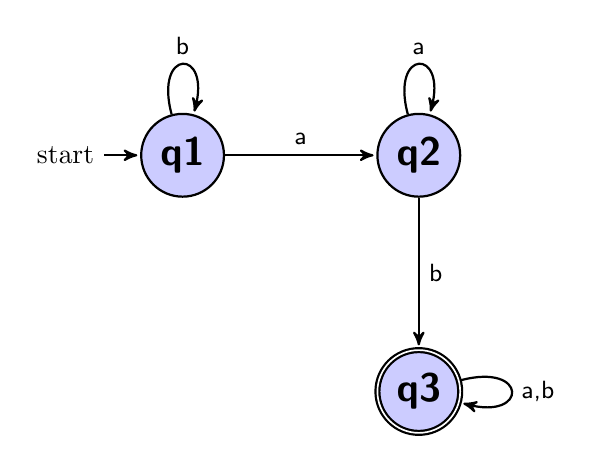
\begin{tikzpicture}[->,>=stealth',shorten >=1pt,auto,node distance=3cm,
  thick,main node/.style={circle,fill=blue!20,draw,font=\sffamily\Large\bfseries}]
  \node[main node, initial] (1) {q1};
  \node[main node] (2) [right of=1] {q2};
  \node[main node, accepting] (3) [below of=2] {q3};
  \path[every node/.style={font=\sffamily\small}]
    (1) edge[loop above] node [above]{b} (1)
        edge node [above]{a} (2)
    (2) edge [loop above] node [above]{a} (2)
        edge node [right] { b } (3)
    (3) edge [loop right] node [right]{ a,b } (3);        
  \end{tikzpicture}
\caption{Constains ab as a substring.}
DFA = \{\{q1, q2, q3\}, \{a, b\}, \{(q1, b) $->$ q1, (q1, a) $->$ q2, (q2, a) $->$ q2, (q2, b) $->$ q3, (q3, b) $->$ q3, (q3, a) $->$ q3\}, q1, \{q3\}\}
\endminipage\hfill
\minipage{0.32\textwidth}
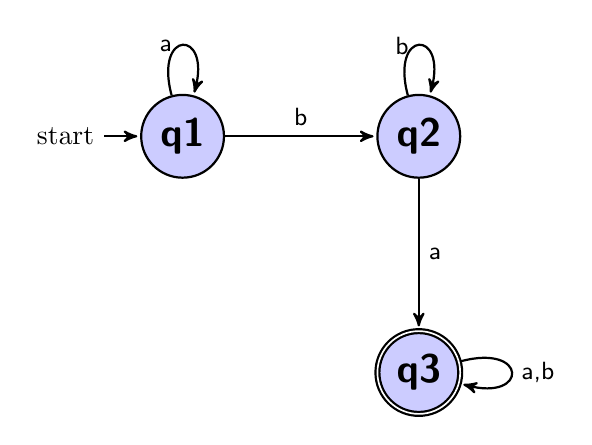
\begin{tikzpicture}[->,>=stealth',shorten >=1pt,auto,node distance=3cm,
  thick,main node/.style={circle,fill=blue!20,draw,font=\sffamily\Large\bfseries}]
  \node[main node, initial] (1) {q1};
  \node[main node] (2) [right of=1] {q2};
  \node[main node, accepting] (3) [below of=2] {q3};
  \path[every node/.style={font=\sffamily\small}]
    (1) edge[loop above] node [left]{a} (1)
        edge node [above]{b} (2)
    (2) edge [loop above] node [left]{b} (2)
        edge node [right] {a} (3)
    (3) edge [loop right] node [right]{a,b} (3);
  \end{tikzpicture}
\caption{Constains ba as a substring}
DFA = \{\{q1, q2, q3\}, \{a, b\}, \{(q1, a) $->$ q1, (q1, b) $->$ q2, (q2, b) $->$ q2, (q2, a) $->$ q3, (q3, a) $->$ q3, (q3, b) $->$ q3\}, q1, \{q3\}\}  
\endminipage\hfill
\end{figure}
\begin{figure}[H]
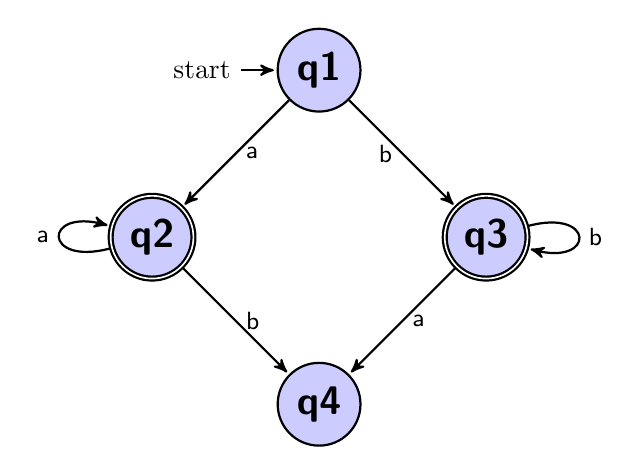
\begin{tikzpicture}[->,>=stealth',shorten >=1pt,auto,node distance=3cm,
  thick,main node/.style={circle,fill=blue!20,draw,font=\sffamily\Large\bfseries}]
  \node[main node, initial] (1) {q1};
  \node[main node, accepting] (2) [below left of=1] {q2};
  \node[main node, accepting] (3) [below right of=1] {q3};
  \node[main node] (4) [below right of=2] {q4};
  \path[every node/.style={font=\sffamily\small}]
    (1) edge node [right]{a} (2)
        edge node [left]{b} (3)
    (2) edge [loop left] node [left]{a} (2)
        edge node [right] {b} (4)
    (3) edge [loop right] node [right]{b} (3)
        edge node [right] {a} (4);
 \end{tikzpicture}
\caption{Constains neither the substrings ab nor ba}
\end{figure}
\section*{Question 2b}
\begin{figure}[H]
\minipage{0.32\textwidth}
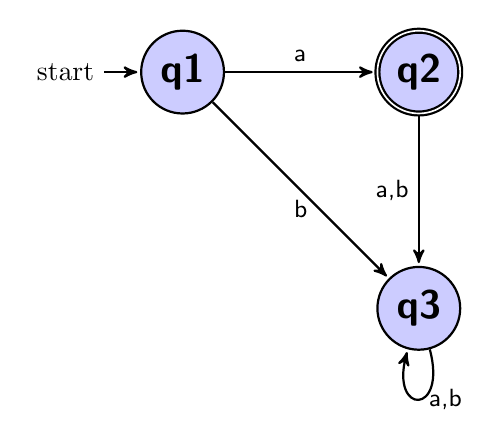
\begin{tikzpicture}[->,>=stealth',shorten >=1pt,auto,node distance=3cm,
  thick,main node/.style={circle,fill=blue!20,draw,font=\sffamily\Large\bfseries}]
  \node[main node, initial] (1) {q1};
  \node[main node, accepting] (2) [right of=1] {q2};
  \node[main node] (3) [below of = 2]{q3};
  \path[every node/.style={font=\sffamily\small}]
    (1) edge node [above]{a} (2)
	edge node [below]{b} (3)
    (2) edge [below] node [left]{a,b} (3)
    (3) edge [loop below] node [right] {a,b}(3);
  \end{tikzpicture}
\caption{Only allows the string a}
\endminipage\hfill
\minipage{0.32\textwidth}
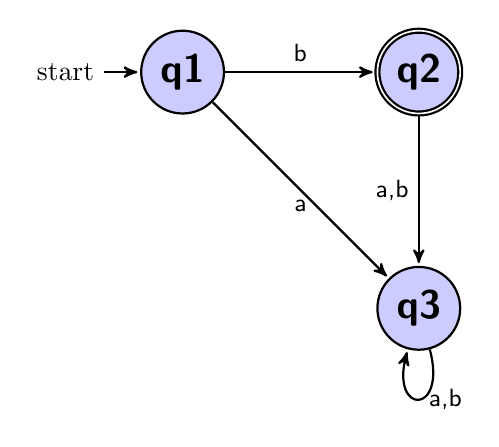
\begin{tikzpicture}[->,>=stealth',shorten >=1pt,auto,node distance=3cm,
  thick,main node/.style={circle,fill=blue!20,draw,font=\sffamily\Large\bfseries}]
  \node[main node, initial] (1) {q1};
  \node[main node, accepting] (2) [right of=1] {q2};
  \node[main node] (3) [below of = 2]{q3};
  \path[every node/.style={font=\sffamily\small}]
    (1) edge node [above]{b} (2)
        edge node [below]{a} (3)
    (2) edge [below] node [left]{a,b} (3)
    (3) edge [loop below] node [right] {a,b}(3);
  \end{tikzpicture}
\caption{Only allows the string b}
\endminipage\hfill
\end{figure}
\begin{figure}[H]
\minipage{0.32\textwidth}
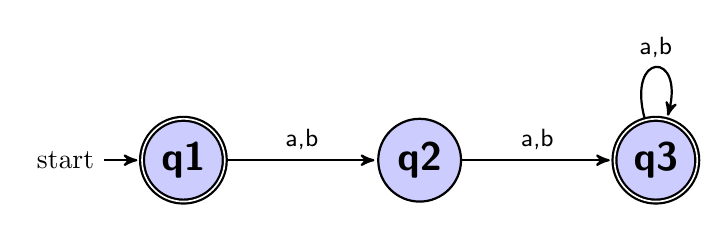
\begin{tikzpicture}[->,>=stealth',shorten >=1pt,auto,node distance=3cm,
  thick,main node/.style={circle,fill=blue!20,draw,font=\sffamily\Large\bfseries}]
  \node[main node, initial, accepting] (1) {q1};
  \node[main node] (2) [right of=1] {q2};
  \node[main node, accepting] (3) [right of = 2]{q3};
  \path[every node/.style={font=\sffamily\small}]
    (1) edge node [above]{a,b} (2)
    (2) edge node [above]{a,b} (3)
    (3) edge [loop above] node [above] {a,b}(3);
  \end{tikzpicture}
\caption{Allowing any strings except a and b}
\endminipage\hfill
\end{figure} 
\section*{Question 3a}
\begin{figure}[H]
\minipage{0.32\textwidth}
  
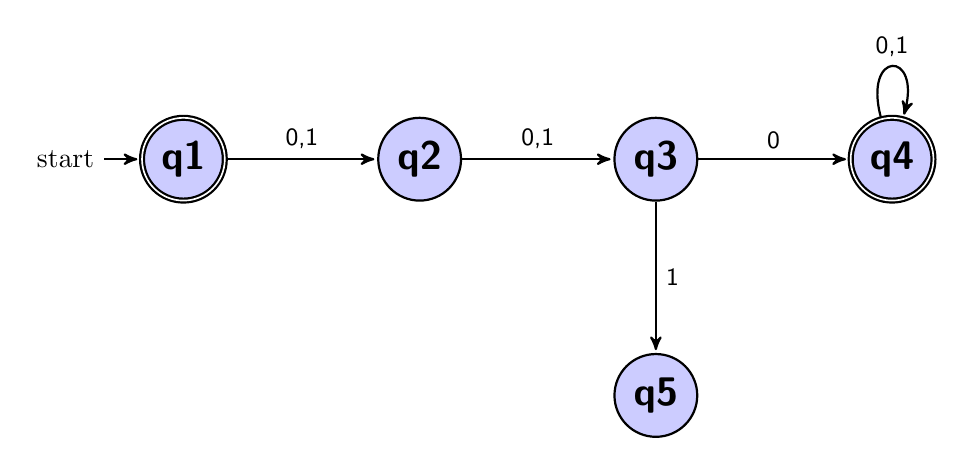
\begin{tikzpicture}[->,>=stealth',shorten >=1pt,auto,node distance=3cm,
  thick,main node/.style={circle,fill=blue!20,draw,font=\sffamily\Large\bfseries}]
  \node[main node, initial, accepting] (1) {q1};
  \node[main node] (2) [right of=1] {q2};
  \node[main node] (3) [right of = 2]{q3};
  \node[main node, accepting] (4) [right of = 3]{q4};
  \node[main node] (5) [below of = 3] {q5};
  \path[every node/.style={font=\sffamily\small}]
    (1) edge node [above]{0,1} (2)
    (2) edge node [above]{0,1} (3)
    (3) edge node [above]{0} (4)
        edge node [right]{1} (5)
    (4) edge[loop above] node [above]{0,1}(4);
  \end{tikzpicture}
\caption{Has the length of atleast 3 and its third symbol is a 0}
\endminipage\hfill
\end{figure}
\section*{Question 3b}
\begin{figure}[H]
\minipage{0.32\textwidth}
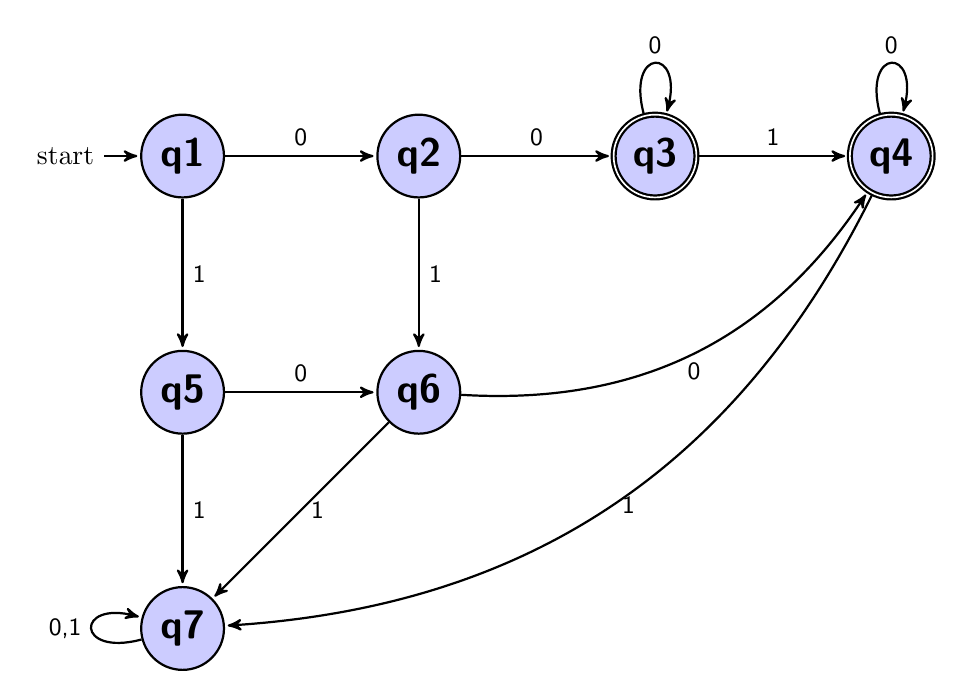
\begin{tikzpicture}[->,>=stealth',shorten >=1pt,auto,node distance=3cm,
  thick,main node/.style={circle,fill=blue!20,draw,font=\sffamily\Large\bfseries}]
  \node[main node, initial] (1) {q1};
  \node[main node] (2) [right of=1] {q2};
  \node[main node, accepting](3) [right of = 2]{q3};
  \node[main node, accepting] (4) [right of = 3]{q4};
  \node[main node] (5) [below of = 1]{q5};
  \node[main node] (6) [below of = 2]{q6};
  \node[main node] (7) [below of = 5]{q7};

  \path[every node/.style={font=\sffamily\small}]
    (1) edge node [above]{0} (2)
	edge node [right]{1} (5)
    (2) edge node [above]{0} (3)
	edge node [right]{1} (6)
    (3) edge node [above]{1}(4)
	edge [loop above] node [above]{0}(3)
    (4) edge [loop above] node [above]{0}(4)
	edge [bend left]node [right]{1}(7)
    (5) edge node[right]{1}(7)
	edge node [above]{0}(6)
    (6) edge [bend right] node [below]{0}(4)
	edge node [right]{1}(7)
    (7) edge [loop left] node [left]{0,1}(7);
  \end{tikzpicture}
\caption{Contains at least two 0s and at most one 1}
\endminipage\hfill
\end{figure}

\end{document}
